%\addbibresource{/home/jorgsk/phdproject/bibtex/jorgsk.bib}

%What results should you present? Anything more than was presented in the paper?

%The figure with the compartments and poly(A)-.

%Shows two things: 1) there is poly(A) signal in poly(A)- extract. explained by
%errors in screening and possibly by short poly(A). 2) intronic polyadenylation in the nucleus overrepresented. Makes
%sense if there is nuclear degradation of intronic poly(A) which has been
%recently shown.

%Then the figure with overlap to show how much you get?

%Then the figure that shows the flattening out of the getting of new
%transcripts.

%Discuss each of the tree figures and that's it.

%Maybe make a table with some of the numbers from the statistics you output.

%Then cite the paper.
\subsection{Summary of the paper}
Summarize the paper.

\subsection{The dataset}
The datasets used in this study was generated by the ENCODE
(\textbf{Enc}yclopedia \textbf{O}f \textbf{D}NA \textbf{E}lements) consortium
and are available from http://hgdownload-test.cse.ucsc.edu/goldenPath/hg19/encodeDCC/wgEncodeCshlLongRnaSeq/

The data is from RNA-seq experiments from 12 human cell lines and their
nuclear and cytoplasmic compartments. Table \ref{tab:Datasets} shows the cell
lines and compartments used; as can be seen, most experiments were available
with a biological replicate. In total, 23 datasets were from whole cell
extracts, 11 were from cytoplasmic extracts, and 12 were from nuclear extracts.
For each cell line and compartment, datasets are available both for the
poly(A)+ and poly(A)- fraction of the RNA pool. This brings the total to 92
RNA-seq datasets. The RNA pool contains only long RNA, that is, RNA over 200
nucleotides in length. Each dataset has been generated with Illumina
paired-ended sequencing with a read-length of 75 basepairs. Each dataset
contains between 150 and 250 million reads.

\begin{table}
	\centering
	\begin{tabular}{cccc}
	  Cell line & Whole Cell & Cytoplasm & Nucleus \\
	  \midrule
	  GM12878 & 2 & 2 & 2 \\
	  K562 & 2 & 2 & 2 \\
	  HeLa-S3 & 2 & 2 & 2 \\
	  HUVEC & 2 & 2 & 2 \\
	  HEPG2 & 2 & 2 & 2 \\
	  H1Hesc & 1 & 1 & 1 \\
	  Nhek & 2 & 0 & 1 \\
	  MCF7 & 2 & 0 & 0 \\
	  AG04450 & 2 & 0 & 0 \\
	  HSMM & 2 & 0 & 0 \\
	  NHLF & 2 & 0 & 0 \\
	  A549 & 2 & 0 & 0 \\
	\end{tabular}
	\caption{Number of replicates of the datasets from the ENCODE consortium}
	\label{tab:Datasets}
\end{table}

The RNA library for this protcol was not especially targeted toward the 3' end
of the RNAs, but since poly(T) primers were used for amplification and cDNA
creation, it is possible to find polyadenylated RNA in these data. What the
data lacks in specificity for the poly(A) sites, it makes up for it in
quantity, with more than 90 datasets from 12 cell lines.

What sets this library apart from most RNA-seq data is that the cell is
compartmentalized and that both the poly(A)+ and poly(A)- fractions of RNA have
been sequenced separately. These extra dimensions increase the resolution of
the data, allowing different hypotheseses to be asked.

\subsection{The short RNA mapper}
The short read mapper used in this work is the GEM mapper
\cite{ribeca_gem_2010}. The GEM mapper is developed in the group of Roderic
Guigo and is production ready, although it has not been published yet.

\section{Results}
We ran Utail on RNA-seq data that was part of the ENCODE consortium. For
details on how Utail works, see the Appendix. Parts of the analysis was
published in XXX. Here we outline our contribution to the paper, including the
parts of the analysis which was not included in the final paper.

\subsection{Total number of polyadenylation sites}
By merging all polyadenylation sites from all samples, a total of XXX
polyadenylation sites were identified. Figure X shows how the number of new
polyadenylation sites saturates as the number of datasets increases. The
saturation is sharper for polyadenylation sites with a downstream PAS,
indicating that ``noisy'' sites increases when the number of reads becomes very
large.

\subsection{Distribution of polyadenylation sites across the genome}
We found that most of the polyadenylation sites are in the 3\p UTR exonic
regions, as expected. The distribution of polyadenylation sites varied between
the whole cell and the cell compartments, see Figure X. Many polyadenylation
sites were found in intergenic regions, indicating sites of transcription
termination at unannotated transcripts.

\subsection{Polyadenylation in the cell's poly(A)- fraction}
We also found evidece for polyadenylated RNA in the poly(A)- fraction. Some of
the sites in the poly(A)- fraction are shared with the poly(A)+ fraction,
indicating that these are sites from RNA that passed the screening proceedure.
Other sites are unique to poly(A)-. Some of these are likely to be noise, as
can be seen from the poly(A)- polyadenylation sites in the cytoplasmic fraction
in Figure X. However, the nuclear fraction shows a strong enrichment of sites
in the poly(A)- fraction compared to the polyA+ fraction, especially in 
intronic regions.

\subsection{Comparison of polyadenylation in the nuclear and cytoplasmic
fractions}
The studies on polyadenylation that have used RNA-seq and microarray
data have so far only used whole cell extracts. Since the RNA in the nucleus
and the cytoplasm are very different, a lot of information is lost by not
considering the two compartments separetely. 

As can be seen in Figure X, the polyadenlyation sites in the cytoplasm have
more support from PET and a higher fraction of them have support by the PAS
hexamer. As well, there is relatively more intronic sites of polyadenylation in
the nucleus for the poly(A)+ fraction as well as the poly(A)- fraction.

\begin{figure}[htb]
	\begin{center}
		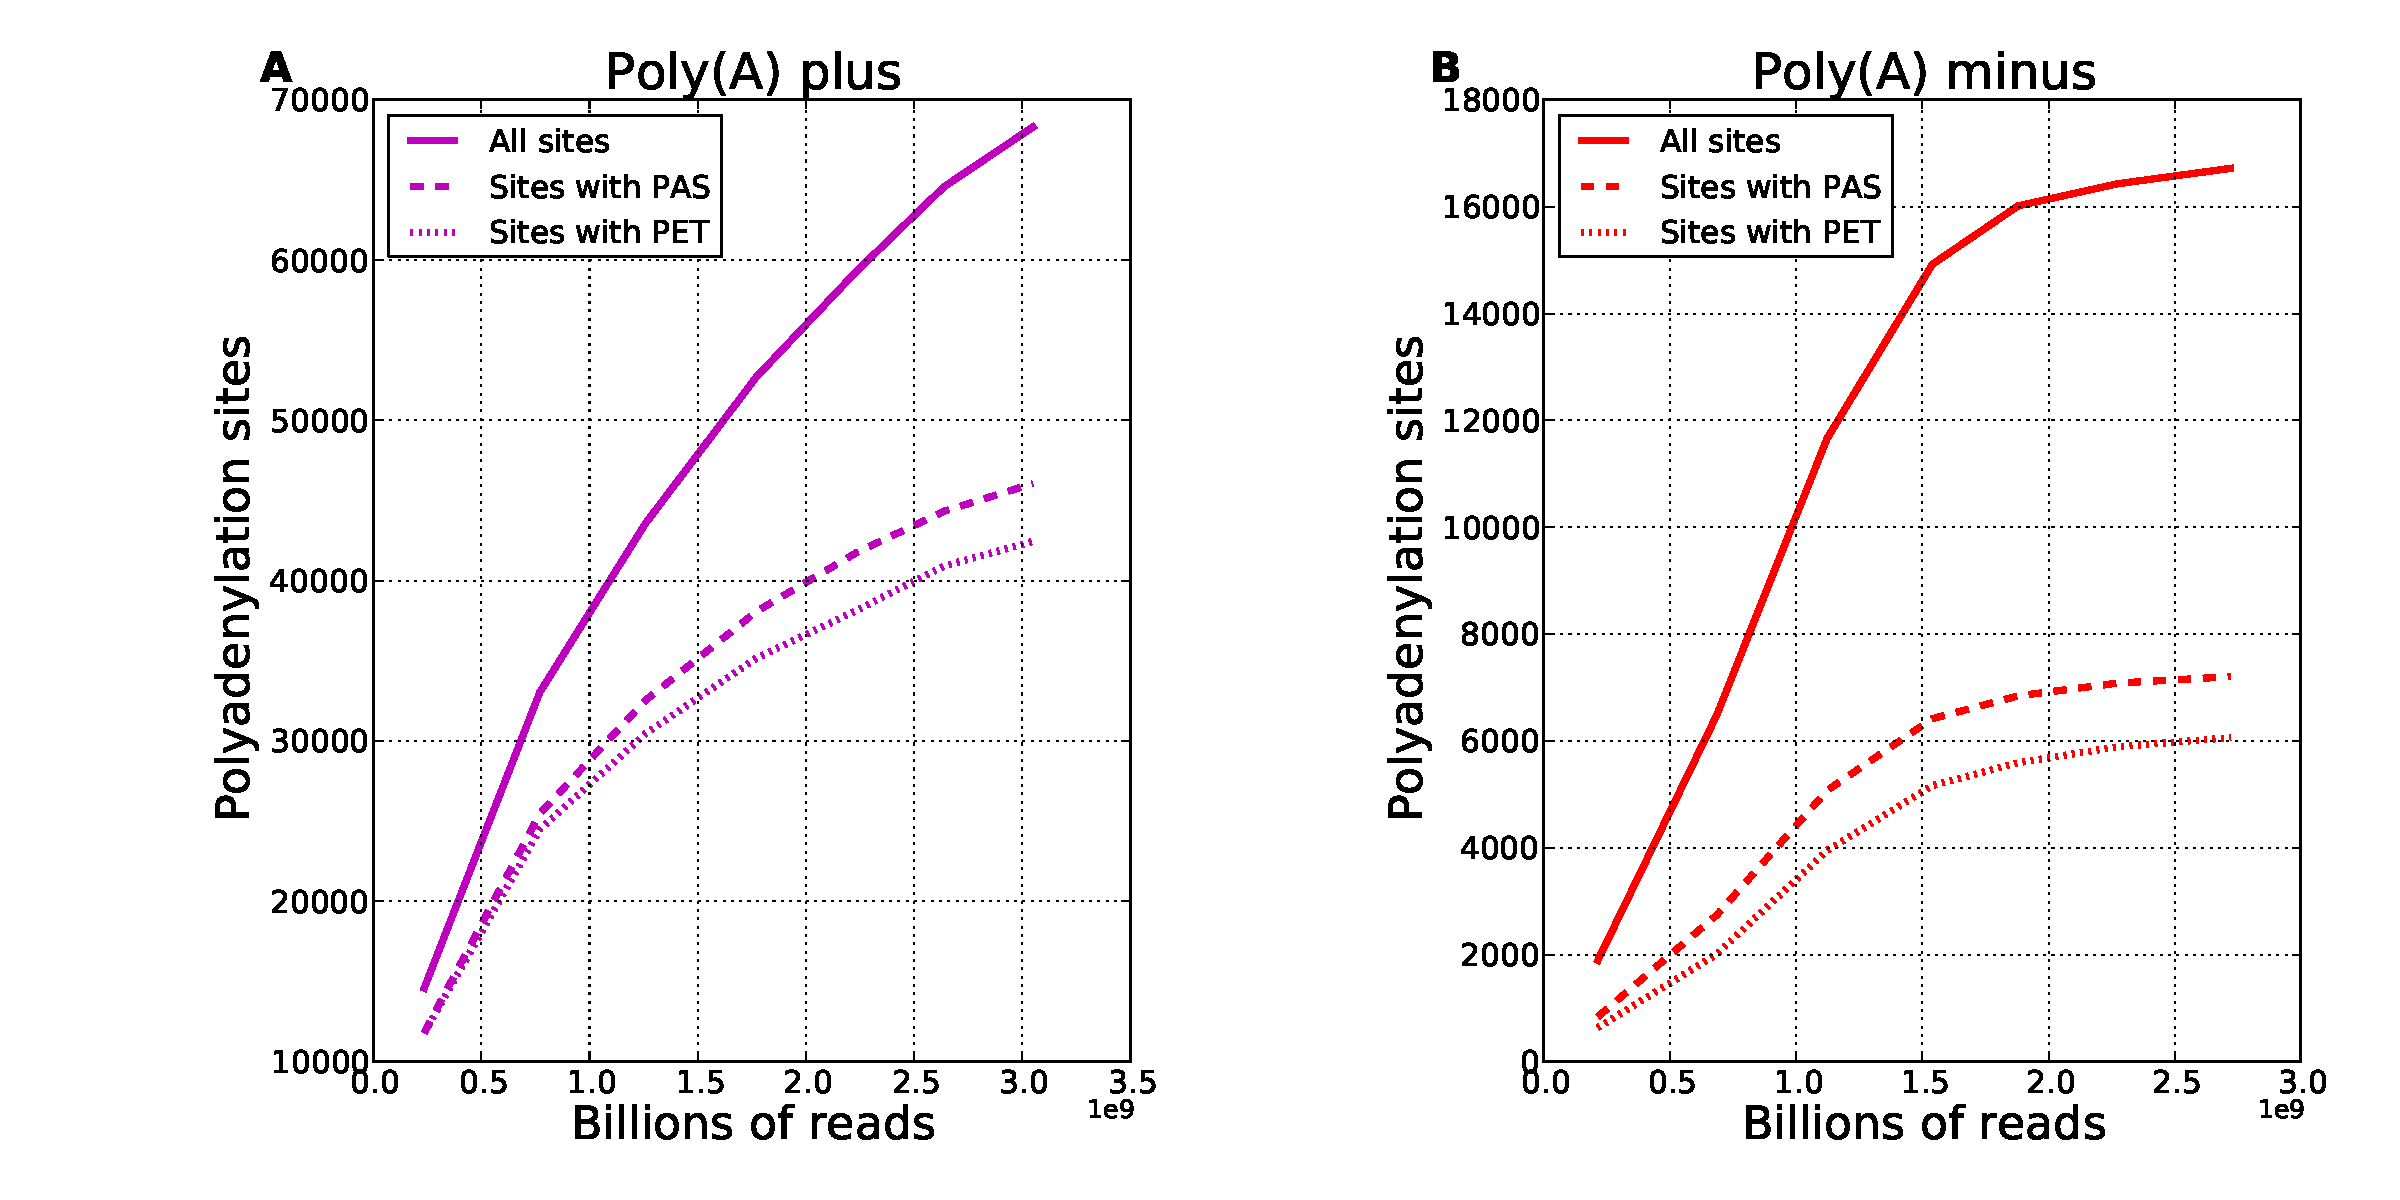
\includegraphics[scale=0.3]{figures/polyadenylation/Saturation_plot_2+.pdf}
	\end{center}
	\caption{Saturation of discovery of polyadenylation sites}
	\label{fig:saturation}
\end{figure}

\begin{figure}[htb]
	\begin{center}
		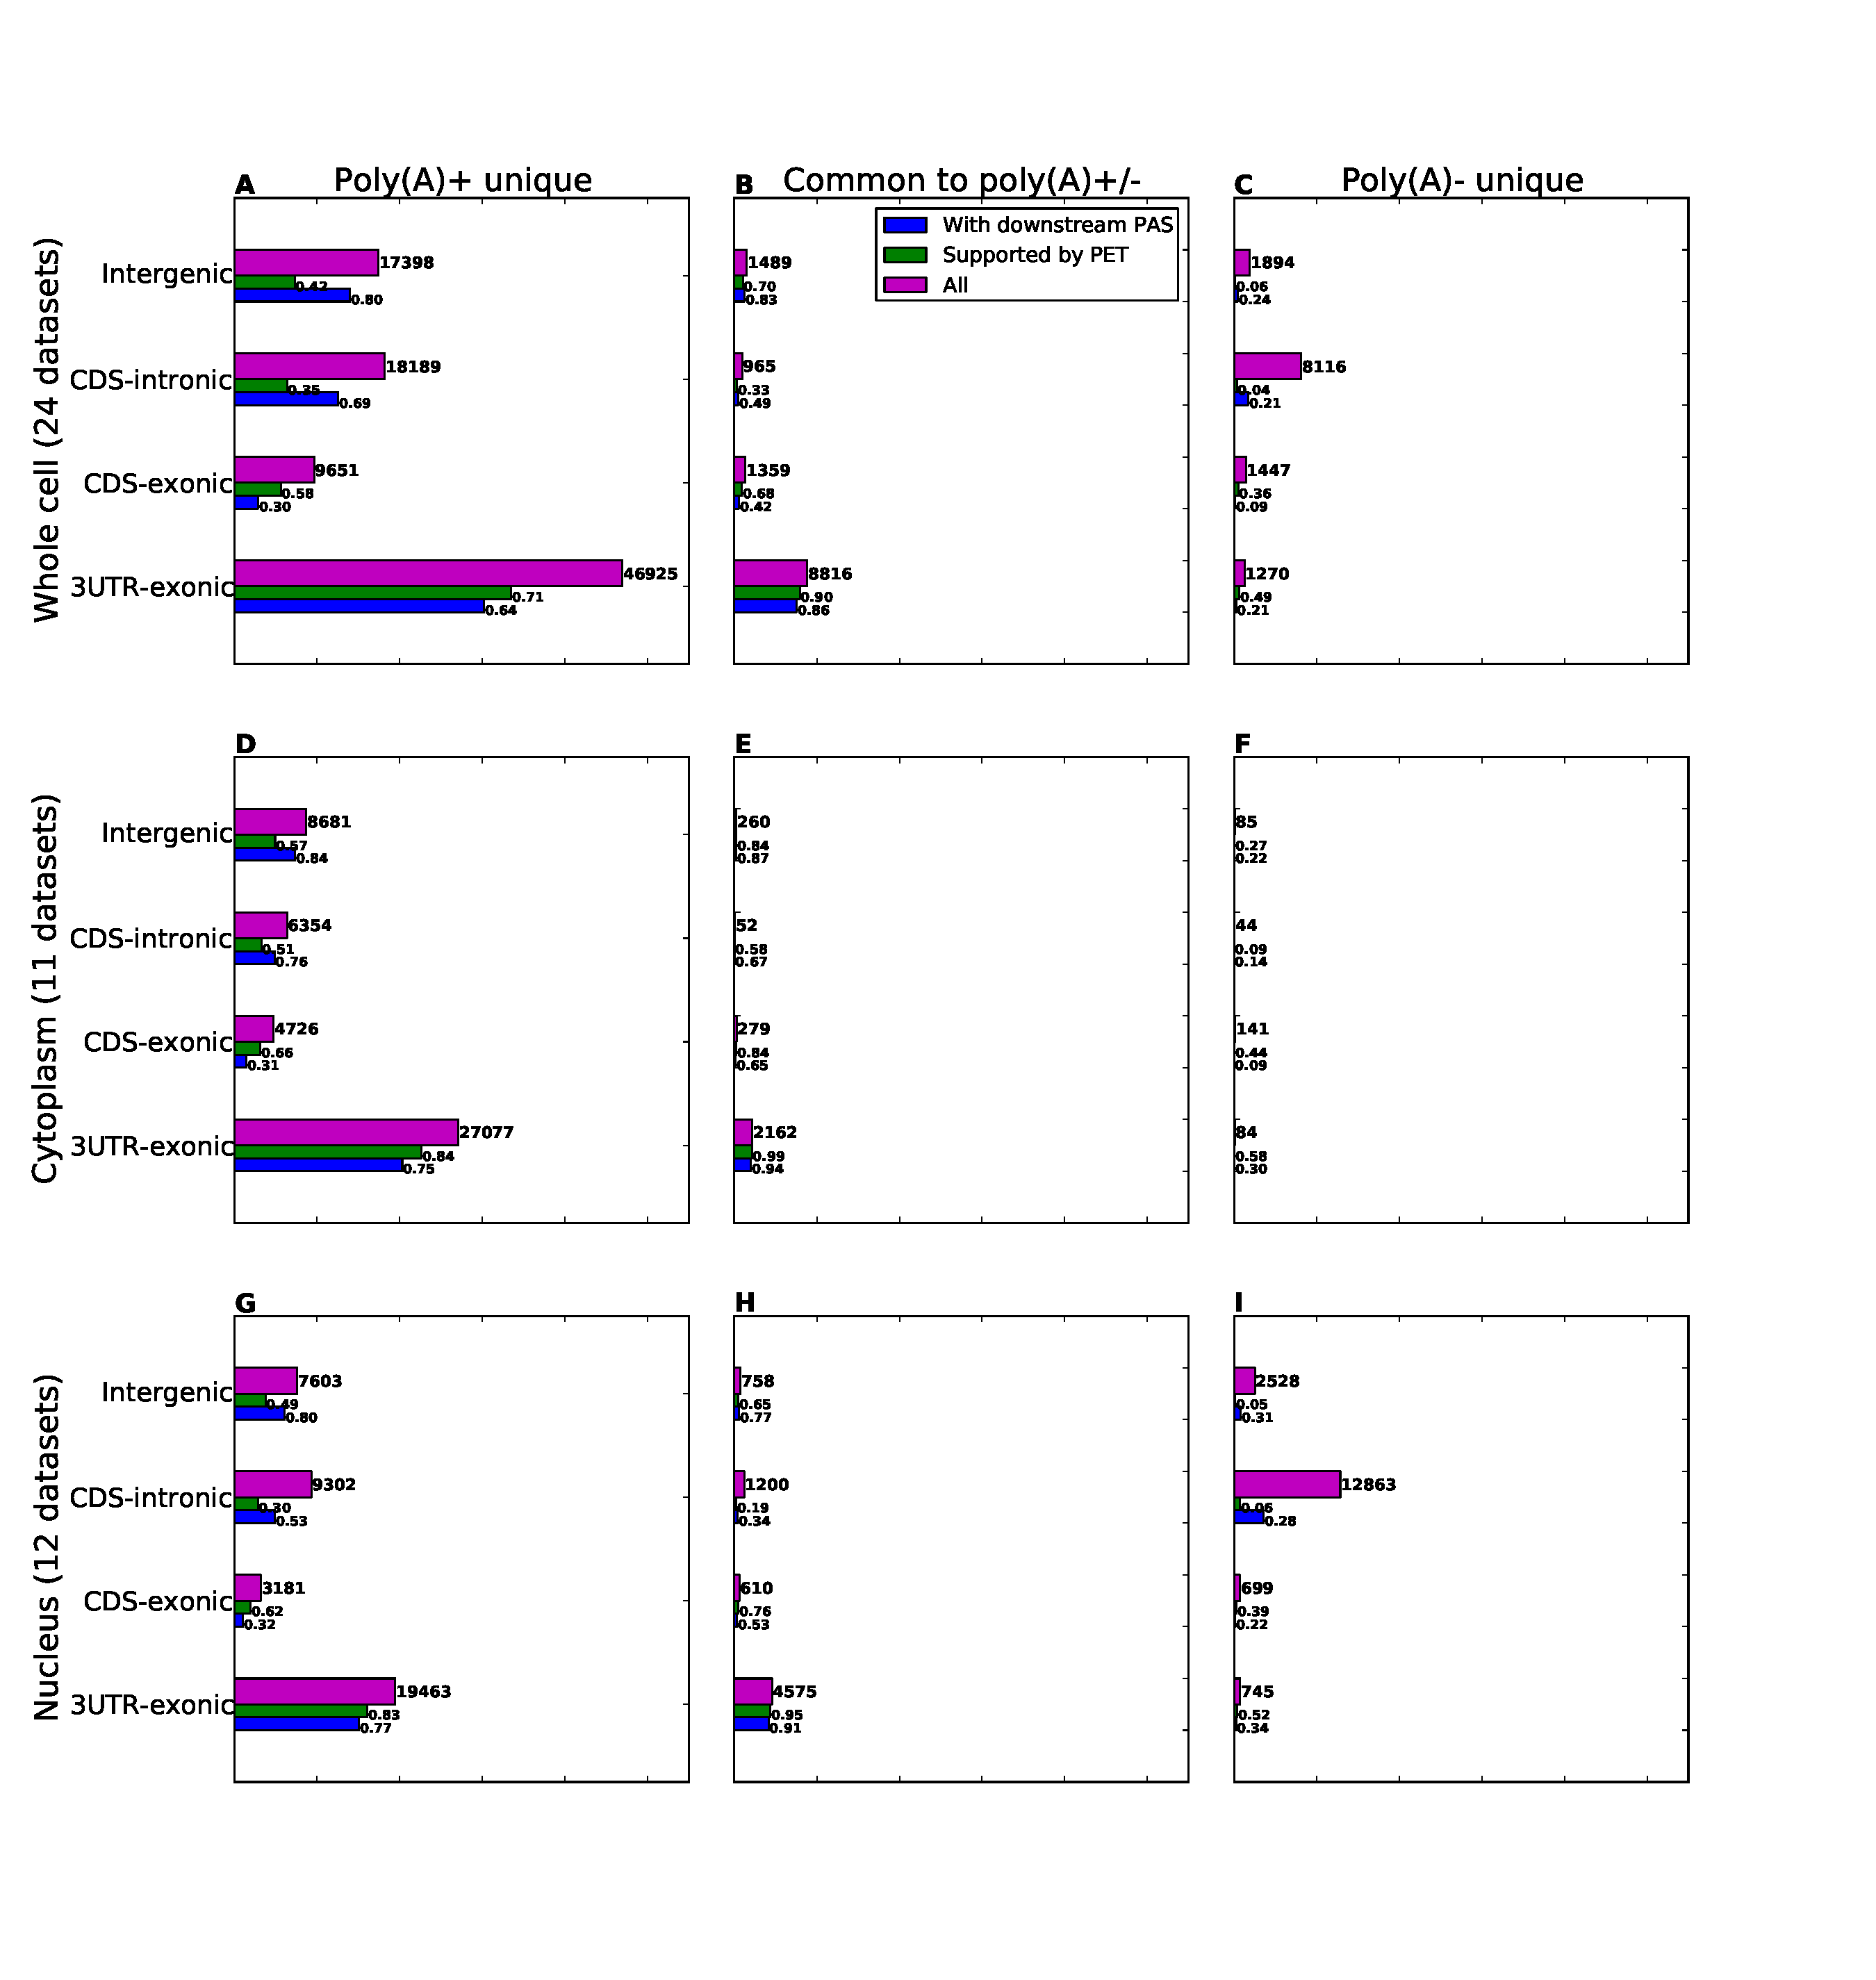
\includegraphics[scale=0.3]{figures/polyadenylation/intersected_sidebars_pA_2+.pdf}
	\end{center}
	\caption{Polyadenylation across genomic regions for the poly(A)+ and poly(A)-
	fractions and the sites that overlap the poly(A)+ and poly(A)- fractions}
	\label{fig:sidebars_intersect}
\end{figure}

\begin{figure}[htb]
	\begin{center}
		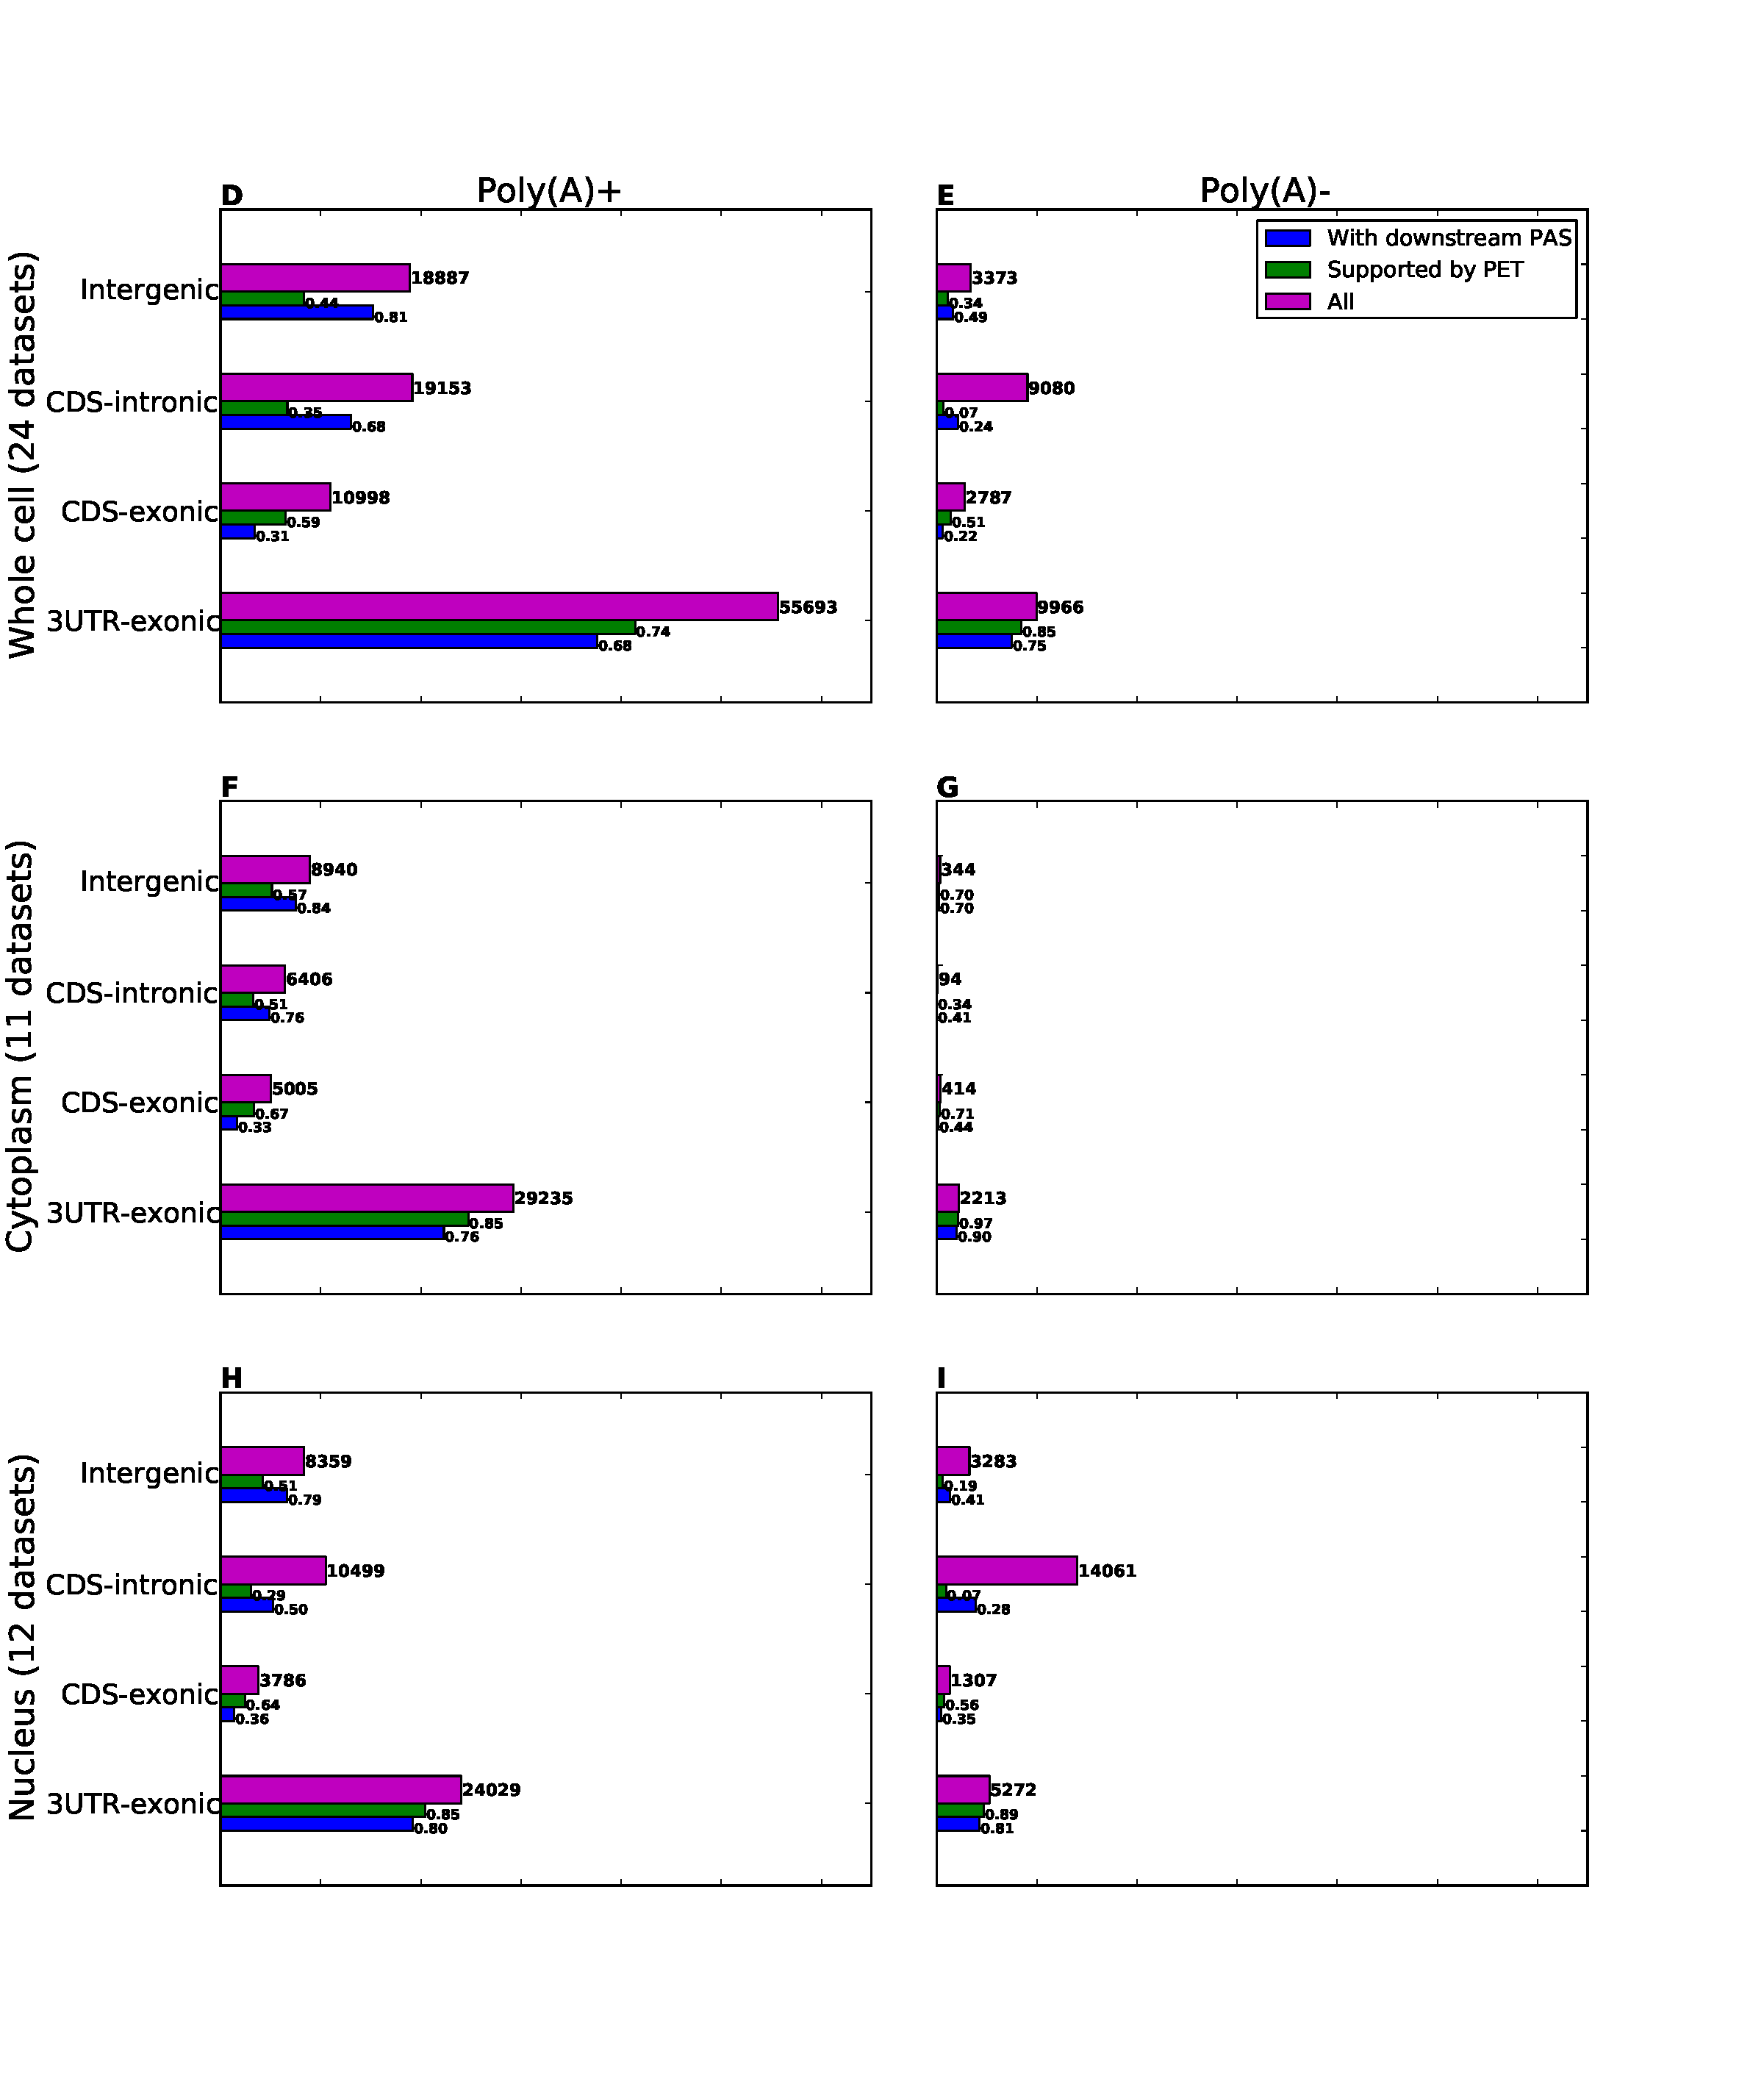
\includegraphics[scale=0.4]{figures/polyadenylation/Sidebars_pA_2+.pdf}
	\end{center}
	\caption{Polyadenylation across genomic regions for the poly(A)+ and poly(A)-
	fractions}
	\label{fig:sidebars}
\end{figure}

TODO! When you re-do the plots, go in and save all the data so you can be
shining on the plots several times without re-doing all the simulations.

\subsubsection{Discussion}
